\section{CausalFusion}


\paragraph{Preliminaries.}\label{sec:background}
We first briefly review the Autoregressive (AR) and Diffusion paradigms in the context of image modeling before introducing our CausalFusion model. Both paradigms factorize the image distribution into a chain of conditional distributions. However, they do so along different axes.
Given a sample of training images $\mathbf{X}$, AR models split $ \mathbf{X} $ along the spatial dimensions into a sequence of tokens, $ \mathbf{X} = \{\mathbf{x}_{1}, \dots, \mathbf{x}_{L}\} $, where $ L $ is the number of tokens. The joint distribution of $ \mathbf{X} $ can be then factorized sequentially:
\begin{equation}\label{eq:AR-factorization}
 q(\mathbf{x}_{1:L}) = q(\mathbf{x}_{1}) \prod_{l=2}^{L} q(\mathbf{x}_{l} | \mathbf{x}_{1:l-1}).
\end{equation}
During training, a neural network $ p_\theta(\mathbf{x}_{l} | \mathbf{x}_{1:l-1}) $ is trained to approximate $ q(\mathbf{x}_{l} | \mathbf{x}_{1:l-1}) $ by minimizing the cross-entropy $ -\mathbb{E}_{q(\mathbf{x}_{1:L})} \log p_\theta(\mathbf{x}_{1:L}) $. At inference time, the image is generated via the \textit{next token prediction} paradigm.

In contrast, Diffusion models gradually add random noise (typically Gaussian) to $\mathbf{X}$ in a so-called \textit{forward process}. It is a Markov chain along the noise level, where each noisy version $\mathbf{x}_t$ is conditioned on the previous state $ \mathbf{x}_{t-1} $ as $ q(\mathbf{x}_t | \mathbf{x}_{t-1}) = \mathcal{N}(\mathbf{x}_t; \sqrt{1 - \beta_t} \mathbf{x}_{t-1}, \beta_t \mathbf{I}) $. Here, $ \beta_t $ is a variance schedule that ensures the forward process starts with a clean image $ \mathbf{x}_0 = \mathbf{X} $ and gradually converges to random noise as $ t \rightarrow T $. The joint distribution of $ \mathbf{X} $ is then factorized as: 
\begin{equation}\label{eq:diffusion-factorization}
q(\mathbf{x}_{0:T}) = q(\mathbf{x}_0)\prod_{t=1}^T q(\mathbf{x}_t | \mathbf{x}_{t-1}).
\end{equation}
To obtain $ \mathbf{X} $ from noise, a neural network is trained to approximate the reverse transition of the forward process for $ t \in [1, T] $:
\begin{equation}\label{eq:diffusion-reverse}
p_\theta(\mathbf{x}_{t-1} | \mathbf{x}_t) = \mathcal{N}(\mathbf{x}_{t-1}; {\mu_\theta}(\mathbf{x}_t), \Sigma_\theta(\mathbf{x}_t))
\end{equation}
As in AR models, training involves minimizing the cross-entropy between $ q(\mathbf{x}_{0:T}) $ and $p_\theta(\mathbf{x}_{0:T})$. 
In DDPM~\cite{ddpm}, $\Sigma_\theta(\mathbf{x}_t)$ is set to a constant value derived from the forward process, and $\mu_\theta(\mathbf{x}_t)$ is set to be the linear combination of $\mathbf{x}_t$ and a noise prediction model $\epsilon_\theta$ that predicts the noise $\mathbf{\epsilon}$ of the forward process. This parameterization leads to the following training objective:
\begin{equation}\label{eq:diffusion_loss}
    \min_\theta \mathbb{E}_{\mathbf{x}_0, \mathbf{\epsilon}, t}[w(t) \|\mathbf{\epsilon} - \epsilon_\theta(\mathbf{x}_t, t)\|^2] 
\end{equation}
where $w(t)$ is derived according to the noise schedule $\beta_t$, which gradually decays as $t$ grows. This objective is further simplified by setting $w(t) = 1$ for all $t$, results in a weighted evidence lower bound that emphasizes more difficult denoising tasks (i.e., larger noise level) at larger $t$ step. 



\begin{figure}[t]
    \centering
    \includegraphics[width=1.02\linewidth]{figs/CasualFusion-arch.pdf}
    \caption{\textbf{Conceptual comparison between the DiT and CausalFusion architectures}. a) DiT incorporates conditioning via adaptive layer normalization, processing a fixed-size set of entire image tokens as input. All the noise tokens $x_t$ are fed into DiT with full attention observation, enabling comprehensive modeling of the input during processing.
    b) CausalFusion treats all input modalities equally in an in-context manner, denoising a random subset of image tokens $x_{t, \kappa_s}$ at each step while causally conditioning on previously denoised tokens $x_{0, 1:\kappa_{s-1}}$, and other contextual inputs. This approach enforces the model to reconstruct the image with partial observation, embodying the spirit of masked feature prediction models \cite{he2022masked, maskedpredict, flip}.
    \vspace{-5pt}
    }
    \label{fig:arch}
\end{figure}



\paragraph{Our approach.}
From the above formulations, the AR and diffusion paradigms naturally support the scaling of sequence length and denoising steps, respectively, offering complementary advantages for image generation. To unify their advantages, we present CausalFusion, a general paradigm that scales effectively in both directions. 

We start by directly extending Eqn.~(\ref{eq:diffusion-factorization}) to encompass the AR factorization:
\begin{align}\label{eq:cd-factorization}
& q(\mathbf{x}_{0:T,\kappa_s} | \mathbf{x}_{0,\kappa_{1:s-1}}) = \nonumber \\ 
& q(\mathbf{x}_{0,\kappa_s}) \prod_{t=1}^T q(\mathbf{x}_{t,\kappa_s} | \mathbf{x}_{t-1,\kappa_s},\mathbf{x}_{0,\kappa_{1:s-1}}) \tag{5}
\end{align}
for $s \in [1, S]$. Here, $S$ denotes the total number of AR steps, while $\kappa_s$ is an index set that identifies the subset of image tokens to be processed at the $s$-th AR step, with $|\kappa_s|$ representing the number of tokens in this subset. Each AR step processes only the tokens indicated by $\kappa_s$, isolating specific portions of the image, as shown in the top row of Figure~\ref{fig:dual-factorization}. The term $\mathbf{x}_{t,\kappa_s}$ represents the dual-factorized image tokens at the $s$-th AR step and $t$-th diffusion step.

During training, the objective of our CausalFusion model is to approximate $p_\theta(\mathbf{x}_{t-1,\kappa_s} | \mathbf{x}_{t,\kappa_s},\mathbf{x}_{0,\kappa_{1:s-1}})$ for all $t$ and $s$. Compared with the formulation in Eqn.~(\ref{eq:diffusion-reverse}),
CausalFusion requires the training sequence to contain not only noised image tokens at the current AR step $\mathbf{x}_{t,\kappa_s}$, but also the clean image tokens from all previous AR steps $\mathbf{x}_{0,\kappa_{1:s-1}}$, allowing the model to leverage information from earlier AR steps to refine the current tokens effectively.
A generalized version of causal attention mask is also required to prevent $\mathbf{x}_{0,\kappa_{1:s-1}}$ from observing $\mathbf{x}_{t,\kappa_s}$.
During inference, the dual-factroization in Eqn.~(\ref{eq:cd-factorization}) enables CausalFusion to generate an unlimited sequence of image tokens through a \textit{next token(s) diffusion} approach while enhancing the quality of each token by applying larger numbers of diffusion steps. See Figure~\ref{fig:arch}(b) for an illustration of CausalFusion model architecture. Further details on the generalized causal attention mask can be found in Appendix~\ref{appendix:secA}.

Notably, adhering to the principle of \textbf{minimal inductive bias}, CausalFusion imposes no restrictions on the number of AR steps $S$, the number of tokens processed at each AR step $|\kappa_s|$, or the specific token indices within each AR step. This flexibility enables a broad exploration space for generative modeling in both training and inference stages.

\begin{table}[t]
\footnotesize
\centering
\begin{tabular}{l|cc}
Model & Params (M) & FID10k$\downarrow$ \\ 
\shline
\underline{DiT}~\cite{dit} & 458 & {18.24}  \\
\hline
{- AdaLN-zero}~\cite{dit} & {305} & {26.71} \\
~~+ new recipe & 305 & {21.94}   \\
~~~~+ T embedding & 308 & {20.68}  \\
~~~~~~+ QK-norm & 308 & {18.66} \\
~~~~~~+ lr warmup & 308 & 17.11 \\
\hline
\colorbox{gray!30}{+ All} (In-context DiT) & 308 &  \textbf{13.78}
\end{tabular}
\caption{\textbf{In-context DiT baseline}. ImageNet 256$\times$256, 240 epoch. Baseline settings are marked by \underline{underlines} and selected settings highlighted in \colorbox{gray!30}{gray}.
\vspace{-6pt}
}
\label{tab:in-context-dit}
\end{table}

\section{Initial studies on CausalFusion}\label{sec:init_exps}
To systematically study the design space of CausalFusion, we conduct experiments on the ImageNet dataset~\cite{deng2009imagenet}, where we train class-conditional image generation models at 256$\times$256 resolution. We use the DiT-L/2 model as our base configuration. All models are trained with 240 epochs and evaluated using FID-10k (unless specified, we use FID-10K and FID interchangeably) and the ADM~\cite{adm} codebase. 
Detailed training recipes and model configurations are provided in Appendix~\ref{appendix:secC}.

\begin{figure*}[t]
  \centering
    \begin{subfigure}{0.32\textwidth}
        \centering
        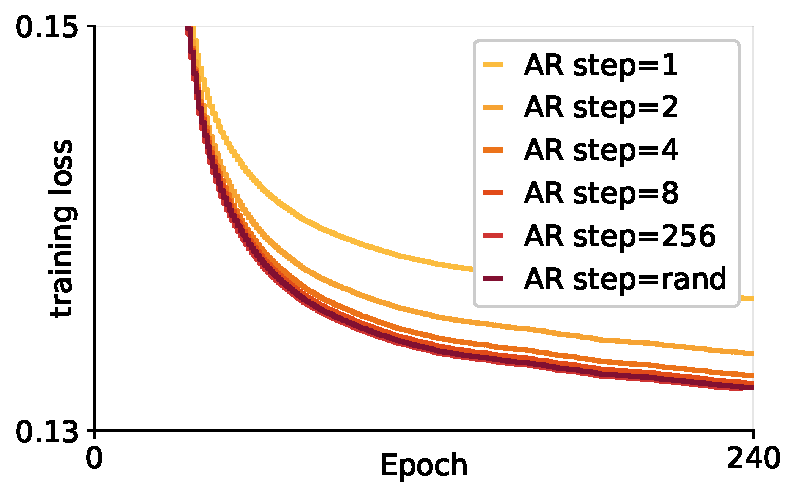
\includegraphics[width=\linewidth]{figs/fig4a.pdf}
        \caption{}
        \label{fig:fig1}
    \end{subfigure}
    \hfill
    \begin{subfigure}{0.32\textwidth}
        \centering
        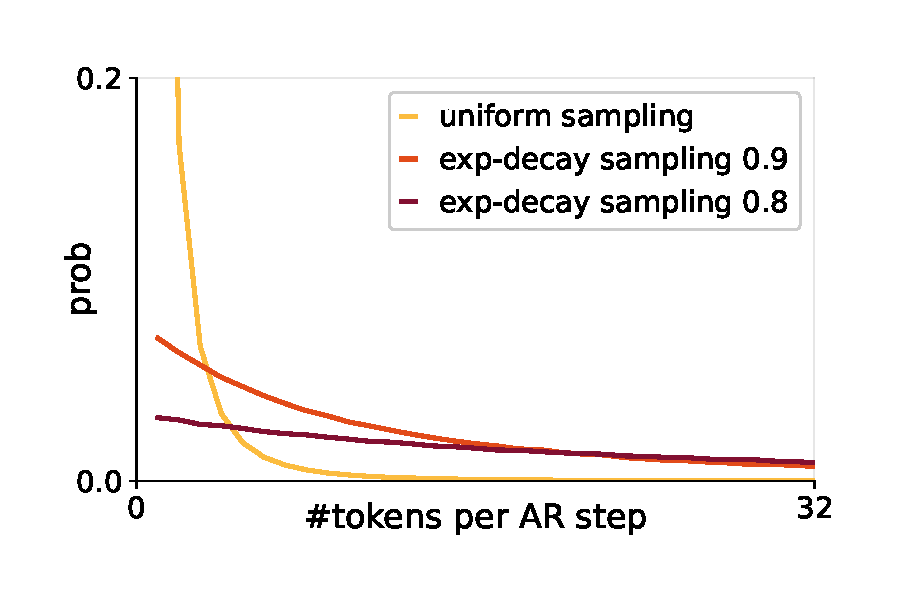
\includegraphics[width=\linewidth]{figs/fig4b-new.pdf}
        \caption{}
        \label{fig:fig2}
    \end{subfigure}
    \hfill
    \begin{subfigure}{0.32\textwidth}
        \centering
        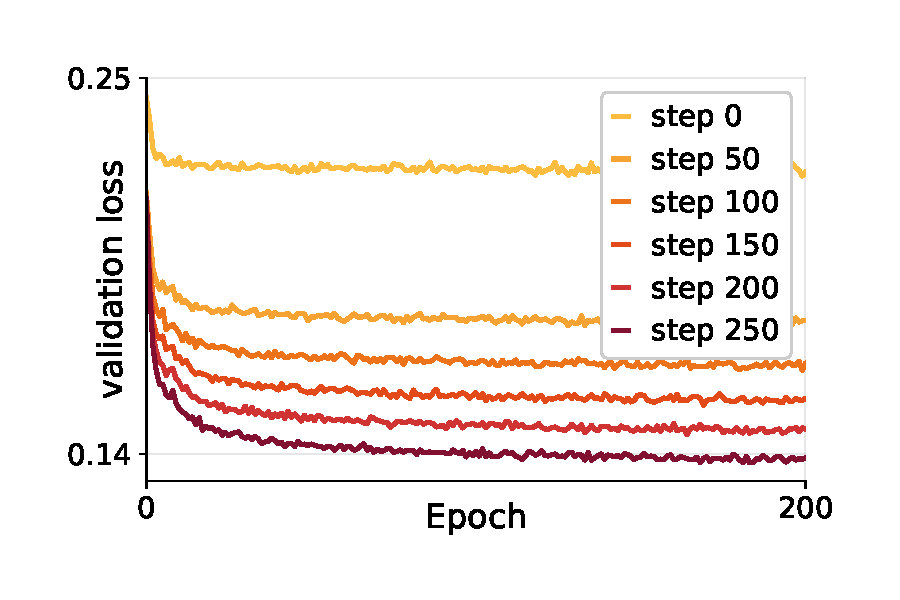
\includegraphics[width=\linewidth]{figs/fig4c.pdf}
        \caption{}
        \label{fig:fig3}
    \end{subfigure}
   \vspace{-5pt}
   \caption{
   (a) Training loss using different number of AR steps. (b) Distribution of $|\kappa_s|$. (c) Validation loss at difference AR steps. 
   \vspace{-6pt}
   }
   \label{fig:weighting_and_decay}
\end{figure*}

\paragraph{Baseline setup: In-context DiT.} As our target is to unify the AR and Diffusion paradigms, we need to unify their architectures first. To this end, we begin with the Transformer-based DiT~\cite{dit} model. Following the DiT design, the 256$\times$256 images are encoded into 32$\times$32 latent representations~\cite{rombach2022high} using a pretrained VAE model, followed by a 2$\times$2 patchify layer that produces a sequence of $L$ = 256 latent tokens. In original DiT, conditional information (e.g., label class) and the diffusion time step are incorporated through AdaLN-zero components, which are incompatible with decoder-only LLMs. To address this limitation, we adopt the in-context design of DiT from~\cite{dit}, treating the class and time step conditions as tokens and directly append them to the image token sequence. By default, we use 4 class tokens and one time step token. As a byproduct, this modification reduces the model size of in-context DiT to approximately $\frac{2}{3}$ of the AdaLN-zero version.

To accelerate training, we use large batch sizes (e.g., 2048) and implement several improvements to stabilize training: (1) injecting the diffusion time step by adding a time step embedding to the image token embeddings instead of using a time step token; (2) applying head-wise QK layer normalization within the self-attention layers, following the practices in~\cite{dehghani2023vit22b}; and (3) incorporating a learning rate warmup stage during training. 

The impact of our new designs is shown in Table~\ref{tab:in-context-dit}. Initially, the native In-context DiT from~\cite{dit} performs significantly worse than the AdaLN-zero version. Our revised training recipe improves performance to 21.94 FID. Incorporating the time step embedding and head-wise QK norm further enhances performance, achieving an FID of 18.66. Adding the learning rate warmup yields an additional improvement. Overall, our final in-context DiT-L/2 model, though conceptually simple, reaches an FID-10k of 13.78—competitive to the best-performing DiT-XL/2 model (12.92 FID-10k) in~\cite{dit}—and serves as a robust baseline that can be steadily trained with large batch sizes.

\begin{table}[t]
\footnotesize
\centering
\begin{tabular}{c|cccc}
 & \multicolumn{4}{c}{FID10k$\downarrow$} \\ 
\#AR steps  & $S_\text{eval}$ = 1 & $S_\text{eval}$ = 2 & $S_\text{eval}$ = 4 & $S_\text{eval}$ = 8\\ 
\shline
\underline{$S_\text{train}$ = 1} & \textbf{13.78} & 356.69 & 404.67 & 390.18 \\ 
$S_\text{train}$ = 2  & 16.69 & \textbf{14.77} & 47.49 & 136.04 \\
$S_\text{train}$ = 4  & 24.14 & 15.37 & \textbf{18.13} & 33.14\\
$S_\text{train}$ = 8  & 54.08 & 24.49 & 22.66 & \textbf{20.01}  \\
$S_\text{train}$ = 256 & 313.28 & 321.62 & 261.26 & 192.25 \\
\hline
\colorbox{gray!30}{random} & 21.31 & 22.17 & 23.54 & 25.05
\end{tabular}
\caption{\textbf{Ablations on AR steps}. $S_\text{train}$ and $S_\text{eval}$ indicates the fixed AR steps used during training and inference, respectively. Baseline settings are marked by \underline{underlines} and selected settings highlighted in \colorbox{gray!30}{gray}.
\vspace{-10pt}
}
\label{tab:ng}
\end{table}


\begin{table*}[t]
\footnotesize
\centering
\subfloat[\textbf{Exponential decay} in AR step sampling. A proper decay ratio leads to competitive or better performance across all inference settings than using fixed AR steps.]{
\begin{tabular}{c|cccc}
 & \multicolumn{4}{c}{FID10k$\downarrow$} \\ 
 {ratio}   & $S_\text{eval}$ = 1 & $S_\text{eval}$ = 2 & $S_\text{eval}$ = 4 & $S_\text{eval}$ = 8 \\ 
\shline
\underline{1.0} & 21.31 & 22.17 & 23.54 & 25.05\\
0.95 & {14.49} & 17.78 & 19.79 & 23.93\\
\colorbox{gray!30}{0.9} &  {12.89} & 15.57 & \textbf{18.83} & \textbf{22.72} \\
0.85 & 12.94 & 15.54 & 19.12 & 23.46\\
0.8 & \textbf{12.78} & \textbf{15.42} & 19.38 & 23.78\\
\end{tabular}
}
\hfill
\subfloat[\textbf{Token order} influences the locality of image tokens and further affects training difficulty.]{
\begin{tabular}{c|c}
Patch order & FID10k$\downarrow$ \\ 
\shline
raster order & {14.46} \\
block-wise raster (8x8) & 14.76 \\
block-wise raster (4x4) & 14.62 \\
dilated order & 15.54 \\
\colorbox{gray!30}{\underline{random order}} & {\textbf{12.89}} \\
\end{tabular}
}
\hfill
\subfloat[\textbf{AR loss weighting} boosts performance by facilitating better learning from difficult samples.]{
\footnotesize
\centering
\begin{tabular}{c|ccc}
 & \multicolumn{3}{c}{FID10k$\downarrow$} \\ 
weight & $S_\text{eval}$ = 1 & $S_\text{eval}$ = 2 & $S_\text{eval}$ = 4 \\ 
\shline
\underline{1$\rightarrow$1} & {12.89} & 15.57 & 18.83 \\
1.5$\rightarrow$1 & {12.61} & 15.49 &  18.32 \\
\colorbox{gray!30}{2$\rightarrow$1} & {\textbf{12.13}} & \textbf{15.15} & 18.09\\
2.5$\rightarrow$1 & {12.32} & 15.22 & 17.99 \\
3$\rightarrow$1 & {12.50} & 15.28 & \textbf{17.92}\\
\end{tabular}
}
\vspace{-5pt}
\caption{\textbf{Ablations on AR step decay, ordering, and AR weighting}. Baseline settings are marked by \underline{underlines} and selected settings highlighted in \colorbox{gray!30}{gray}.
\vspace{-10pt}
}
\label{tab:arweighting}
\end{table*}

\vspace{-5pt}
\paragraph{CausalFusion with fixed number of AR steps.} Building on the In-context DiT baseline, we begin with a simplified version of CausalFusion that uses a fixed number of AR steps $S$ during both training and inference, with the number of tokens predicted at each AR step fixed to $|\kappa_s| = \frac{L}{S}$. Specifically, we modify the input sequence to include clean image tokens and use generalized causal attention masks within the attention modules. Figure~\ref{fig:arch} illustrates the architectural differences between DiT and CausalFusion.
We train several CausalFusion models with different numbers of AR steps, i.e., $S$ = 1, 2, 4, 8, and 256. Here, $S$ = 1 indicates the In-context DiT, while $S$ = 256, equivalent to $L$, represents the pure AR training mode. To evaluate these models, we first use the same number of AR steps as in training, and further study their generalization performance to other number of AR steps. 

As shown in Table~\ref{tab:ng}, CausalFusion trained with fixed AR steps cannot be robustly transferred to other inference settings. E.g., all models yield substantially worse performance when their inference settings are not aligned with training. By comparing the best evaluation result of each training setting, we observe that increasing the number of AR steps leads to a huge decline in performance. Specifically, the 8-step CausalFusion yields an FID of 20.01, clearly lagging behind the 13.78 FID achieved by In-context DiT. However, from the loss curves in Figure~\ref{fig:weighting_and_decay}(a), an opposite trend is observed, where models trained with more AR steps consistently exhibit lower loss values than those with fewer AR steps. This suggests that the learning tasks become over-simplified as the number of AR steps increases.

\vspace{-5pt}
\paragraph{CausalFusion with random number of AR steps.} 
Additionally, we train a CausalFusion model where the number of AR steps $S$ are uniformly sampled from 1 to $L$, with $|\kappa_s|$ also randomly set at each AR step. We evaluate this model across various inference settings, same as above. As shown in Table~\ref{tab:ng}, this training setting performs relatively consistent under different inference AR steps compared to those trained with fixed AR steps, demonstrating its greater flexibility during training and versatility during inference. However, this setting still leads to inferior results compared to the In-context DiT baseline, e.g., an FID of 21.31 when evaluated with a single AR step ($S$ = 1) as diffusion mode. 
Figure~\ref{fig:weighting_and_decay}(b) offers further insight into this behavior, showing that uniform AR step sampling during training leads to a highly imbalanced $|\kappa_s|$ distribution. As a result, the training signal is dominated by AR steps with very few tokens—over 95\% of AR steps have $|\kappa_s| \leq 16$. These steps are uniformly distributed along the AR axis, causing the model to overly rely on visible context and thus diminishing the complexity of the training task.

Lastly, given the CausalFusion model trained with random AR steps, we compare the loss values produced by different AR steps on the validation set. As shown in Figure~\ref{fig:weighting_and_decay}(c), later AR steps yield much lower loss values than earlier steps, suggesting a clear trend of vanished training signals along the AR axis. 

\section{Shaping task difficulties in CausalFusion} \label{sec:difficulty}
Based on the above observations, we aim to adjust the difficulties of the generative tasks in CausalFusion to balance training signal impact and ensure thorough exploration of the factorization space. By default, we use random AR steps during training due to its effectiveness in generalizing across various inference settings. Building on this setup, we identify several straightforward approaches that effectively shape task difficulties within CausalFusion, leading to significant performance improvements. We categorize the discussion into two parts: design choices for AR step sampling and loss weighting along the AR axis. 

\vspace{-5pt}
\paragraph{Random AR steps with decayed sampling.} 
Instead of uniformly sampling the number of AR steps $S$ from $[1, L]$, we propose to exponentially decrease the sampling probability as $S$ increases, which alleviates the problem of imbalanced $|\kappa|_s$ distribution, as shown in Figure~\ref{fig:weighting_and_decay}(b).
As a result, large $|\kappa_s|$ appears more frequently in the training sequence, and more tokens are predicted base on less visible context. We introduce a hyper-parameter $\gamma$ $\leq$ 1 to control the exponential decay ratio where $\gamma$ = 1 denotes the naive CausalFusion model trained with uniformly sampled AR steps, while $\gamma$ = 0 represents our In-context DiT baseline.
From Table~\ref{tab:arweighting}(a), by decreasing $\gamma$ from 1.0 to 0.95, we obtain remarkable performance improvements across all inference settings, with gains of nearly 7 and 5 points when $S_\text{eval}$ = 1 and 2, respectively. Furthermore, when $\gamma$ = 0.9, CausalFusion surpasses the strong In-context DiT using the pure diffusion inference mode, and performance in other inference settings is further enhanced. While smaller values of $\gamma$, such as 0.8, yield even better performance with one AR step evaluation, we set the defualt value to 0.9 as it provides a balanced improvement across all inference settings.


\begin{table*}[t]
\footnotesize
\begin{tabular}{c|c|cccc|cccc|cccc}
& & \multicolumn{4}{c}{256$\times$256, w/o CFG} & \multicolumn{4}{c}{256$\times$256, w/ CFG} & \multicolumn{4}{c}{512$\times$512, w/ CFG}\\
& Params & FID$\downarrow$ & IS$\uparrow$ & Pre.$\uparrow$ & Rec.$\uparrow$ & FID$\downarrow$ & IS$\uparrow$ & Pre.$\uparrow$ & Rec.$\uparrow$ & FID$\downarrow$ & IS$\uparrow$ & Pre.$\uparrow$ & Rec.$\uparrow$ \\
\shline
\textcolor{lightgray}{GIVT~\cite{tschannen2025givt}} & \textcolor{lightgray}{304M} & \textcolor{lightgray}{5.67} & \textcolor{lightgray}{-} & \textcolor{lightgray}{0.75} & \textcolor{lightgray}{0.59} & \textcolor{lightgray}{3.35} & \textcolor{lightgray}{-} & \textcolor{lightgray}{0.84} & \textcolor{lightgray}{0.53} & \textcolor{lightgray}{2.92} & \textcolor{lightgray}{-} & \textcolor{lightgray}{0.84} & \textcolor{lightgray}{0.55} \\
\textcolor{lightgray}{MAR-B~\cite{mar}} & \textcolor{lightgray}{208M} & \textcolor{lightgray}{3.48} & \textcolor{lightgray}{192.4} & \textcolor{lightgray}{0.78} & \textcolor{lightgray}{0.58} & \textcolor{lightgray}{2.31} & \textcolor{lightgray}{281.7} & \textcolor{lightgray}{0.82} & \textcolor{lightgray}{0.57} & \textcolor{lightgray}{-} & \textcolor{lightgray}{-} & \textcolor{lightgray}{-} & \textcolor{lightgray}{-} \\
LDM-4~\cite{rombach2022high} & 400M & 10.56 & 103.5 & 0.71 & 0.62 & 3.6 & 247.7 & \textbf{0.87} & 0.48 & - & - & - & - \\
CausalFusion-L & 368M & \textbf{5.12} & \textbf{166.1} & \textbf{0.73} & \textbf{0.66} & \textbf{1.94} & \textbf{264.4} & 0.82 & \textbf{0.59} & - & - & - & - \\
\hline
\textcolor{lightgray}{MAR-L~\cite{mar}} & \textcolor{lightgray}{479M} & \textcolor{lightgray}{2.6} & \textcolor{lightgray}{221.4} & \textcolor{lightgray}{0.79} & \textcolor{lightgray}{0.60} & \textcolor{lightgray}{1.78} & \textcolor{lightgray}{296.0} & \textcolor{lightgray}{0.81} & \textcolor{lightgray}{0.60} & \textcolor{lightgray}{1.73} & \textcolor{lightgray}{279.9} & \textcolor{lightgray}{-} & \textcolor{lightgray}{-} \\
ADM~\cite{adm} & 554M & 10.94 & - & 0.69 & 0.63 & 4.59 & 186.7 & 0.82 & 0.52 & 3.85 & 221.7 & {0.84} & 0.53 \\
DiT-XL~\cite{dit} & 675M & 9.62 & 121.5 & 0.67 & 0.67 & 2.27 & 278.2 & \textbf{0.83} & 0.57 & 3.04 & 240.8 & {0.84} & 0.54 \\
SiT-XL~\cite{sit} & 675M & 8.3 & - & - & - & 2.06 & 270.3 & 0.82 & 0.59 & 2.62 & 252.2 & \textbf{0.84} & 0.57 \\
ViT-XL~\cite{minsnr} & 451M & 8.10 & - & - & -  & 2.06 & - & - & - & - & - & - & - \\
U-ViT-H/2~\cite{bao2023all} & 501M & 6.58 & - & - & - & 2.29 & 263.9 & 0.82 & 0.57 & 4.05 & - & - & -\\
MaskDiT~\cite{zheng2023fast} & 675M & 5.69 & 178.0 & 0.74 & 0.60 & 2.28 & 276.6 & 0.80 & 0.61 & 2.50 & 256.3 & 0.83 & 0.56 \\
RDM~\cite{teng2023relay} & 553M & 5.27 & 153.4 & 0.75 & 0.62 & 1.99 & 260.4 & 0.81 & 0.58 & - & - & - & - \\
CausalFusion-XL & 676M & \textbf{3.61} & \textbf{180.9} & \textbf{0.75} & \textbf{0.66} & \textbf{1.77} & \textbf{282.3} & 0.82 & \textbf{0.61} & \textbf{1.98} & \textbf{283.2} & 0.83 & \textbf{0.58} \\
\end{tabular}
\vspace{-8pt}
\caption{
\textbf{System performance comparison} on ImageNet class-conditioned generation. Numbers marked with \textcolor{lightgray}{gray} blocks use temperature sampling during inference.
\vspace{-8pt}
}
\label{tab:system}
\end{table*}

\vspace{-5pt}
\paragraph{Loss weighting along AR axis.} We modify the weighting term $w(\cdot)$ in Eqn.~(\ref{eq:diffusion_loss}) to further consider the AR step $s$. In practice, we simply set $w(s, t)$ to a pre-defined value $\lambda \geq 1$ at $s=1$, and linearly decay it to 1 at $s=S$, and keep using constant weight for different $t$. In this way, the model is trained to focus more on the hard generative tasks at early AR steps or larger noise levels.
We analysis the impact of $\lambda$ in Table~\ref{tab:arweighting}(c). From the table, setting $\lambda$ to a proper value improves the performance. Intuitively, as the model generates closer to the end of the AR axis, the task becomes easier due to high \textbf{locality}\cite{wang2018non} in the visible context, causing some generative tasks to degrade into local feature interpolation. 
In contrast, predictions made during earlier AR steps facilitate the learning of non-local dependencies within the visual context, which is beneficial to generative modeling.

\vspace{-5pt}
\paragraph{Difficulty vs. locality.} The hypothesis of {locality} aligns with our observations in Table~\ref{tab:arweighting}(b), where using random sequence order in CausalFusion during training significantly outperforms manually assigned orders. Specifically, using fixed (block-wise) raster order leads the model to rely excessively on local tokens, which makes the training task easier. In contrast, CausalFusion is trained with a random order by default, following the principle of \textit{minimal inductive bias}. This design encourages the model to develop robust generative modeling abilities rather than relying on fixed ordering priors, while allowing flexible inference orders.

\section{Performance comparison}\label{sec:sota_exp}


\begin{table*}[t]
\footnotesize
\begin{tabular}{c|ccccccc}
& Type & Tokenizer & Params & Training Epoch & Sampler (Steps) & Sampling tricks & FID$\downarrow$  \\
\shline
Open-MAGVIT2-L~\cite{luo2024open} & AR & MAGVIT2 & 800M & 300 & AR(256) & N/A  & 2.51 \\
Open-MAGVIT2-XL~\cite{luo2024open} & AR & MAGVIT2 & 1.5B & 300 & AR(256) & N/A  & 2.33 \\
LlamaGen-3B~\cite{sun2024autoregressive} & AR & custom & 3.1B & - & AR(256) & N/A & 2.18 \\
VAR-d24~\cite{tian2024visual} & VAR & custom & 1B & 350 & VAR & N/A  & 2.09\\
VAR-d30~\cite{tian2024visual} & VAR & custom & 2B & 350 & VAR & reject sampling & 1.73 \\
\hline
Simple-diffusion~\cite{hoogeboom2023simple} & Diffusion & N/A & 2B & 800 & DDPM & N/A  & 2.44 \\ 
FiTv2-3B~\cite{wang2024fitv2} & Diffusion & SD & 3B & 256 & DDPM(250) & N/A & 2.15 \\
VDM++~\cite{kingma2024understanding} & Diffusion & N/A & 2B & - & EDM & - & 2.12 \\
Large-DiT-7B~\cite{gao2024lumina} & Diffusion & SD & 3B & 435 & DDPM(250) & N/A & 2.10 \\
Flag-DiT-3B~\cite{gao2024lumina} & Diffusion & SD & 3B & 256 & adaptive Dopri-5 & N/A & 1.96 \\
DiT-MoE-XL/2-8E2A~\cite{fei2024scaling} & Diffusion & SD & 16B & $\approx$1000 & DDPM(250) & N/A & 1.72 \\
DiMR-G/2R~\cite{liu2024alleviating} & Diffusion & SD & 1.1B & 800 & DPM-solver(250) & N/A & 1.63 \\
\hline
DART-XL~\cite{dart} & AR+Diffusion & LDM & 812M & - & AR(256)+FM(100) & $\tau$ sampling & 3.98 \\
MonoFormer~\cite{monoformer} & AR+Diffusion & SD & 1.1B & - & DDPM(250) & N/A & 2.57 \\
BiGR-XL-d24~\cite{bigr} & AR+Diffusion & custom & 799M & 400 & AR(256)+DDPM(100) & $\tau$ sampling  & 2.49 \\
BiGR-XXL-d32~\cite{bigr} & AR+Diffusion & custom & 1.5B & 400 & AR(256)+DDPM(100) & $\tau$ sampling  & 2.36 \\
MAR-H~\cite{mar} & AR+Diffusion & custom & 943M & 800 & AR(256)+DDPM(100) & $\tau$ sampling & 1.55 \\
\hline
CausalFusion-H & Diffusion & custom & 1B & 800 & DDPM(250) & N/A & 1.64 \\
CausalFusion-H & Diffusion & custom & 1B & 800 & DDPM(250) & CFG interval & {1.57} \\
\end{tabular}
\vspace{-5pt}
\caption{
\textbf{System performance comparison} on 256$\times$256 ImageNet generation, compared with previously reported large models.
\vspace{-10pt}
}
\label{tab:system2}
\end{table*}


\paragraph{Class-conditional image generation.}
\label{sec:system}
We evaluate our final method on the ImageNet class-conditional generation benchmark. For system-level comparisons, we use 64 tokens to encode the class condition. The impact of varying the number of class tokens is analyzed in Appendix~\ref{appendix:secB}. We train three sizes of CausalFusion models: CausalFusion-L (368M), CausalFusion-XL (676M), and CausalFusion-H (1B). All models are trained for 800 epochs with a batch size of 2048. By default, we use a single AR step inference with 250 DDPM steps as in DiT~\cite{dit}, and report FID-50k for benchmarking against existing models. Detailed hyperparameters are provided in Appendix~\ref{appendix:secC}. As shown in Table~\ref{tab:system}, on 256$\times$256 image generation, CausalFusion-L achieves an FID-50k of 5.12 without classifier-free guidance~\cite{ho2022classifier} (CFG), outperforming DiT-XL/2 by 4.5 points with 50\% fewer parameters. CausalFusion-XL further improves this result to 3.61, and when using CFG, achieves a state-of-the-art result of 1.77, significantly outperforming strong baselines like DiT and SiT. Additionally, CausalFusion-XL demonstrates effectiveness in high-resolution generation, achieving an FID of 1.98 on 512$\times$512 images with CFG.

We also provide a system-level comparison with existing methods in Table~\ref{tab:system2}. CausalFusion-H achieves an FID of 1.64 using the standard 250-step DDPM sampler, outperforming previous diffusion models with larger model sizes, such as FiTv2-3B~\cite{wang2024fitv2} and Large-DiT-7B~\cite{gao2024lumina}, and achieving comparable results to DiMR-G/2R (1.64 vs. 1.63) despite DiMR-G/2R’s use of a stronger sampler (DPM-solver~\cite{dpm}). By applying the CFG interval~\cite{kynkaanniemi2024applying} approach, CausalFusion-H further improves to an FID of 1.57, positioning it among the top-performing models on the ImageNet 256$\times$256 benchmark.


\begin{figure}[h!]
    \centering
    \vspace{0pt}
    \begin{subfigure}{1\textwidth}
        \centering
        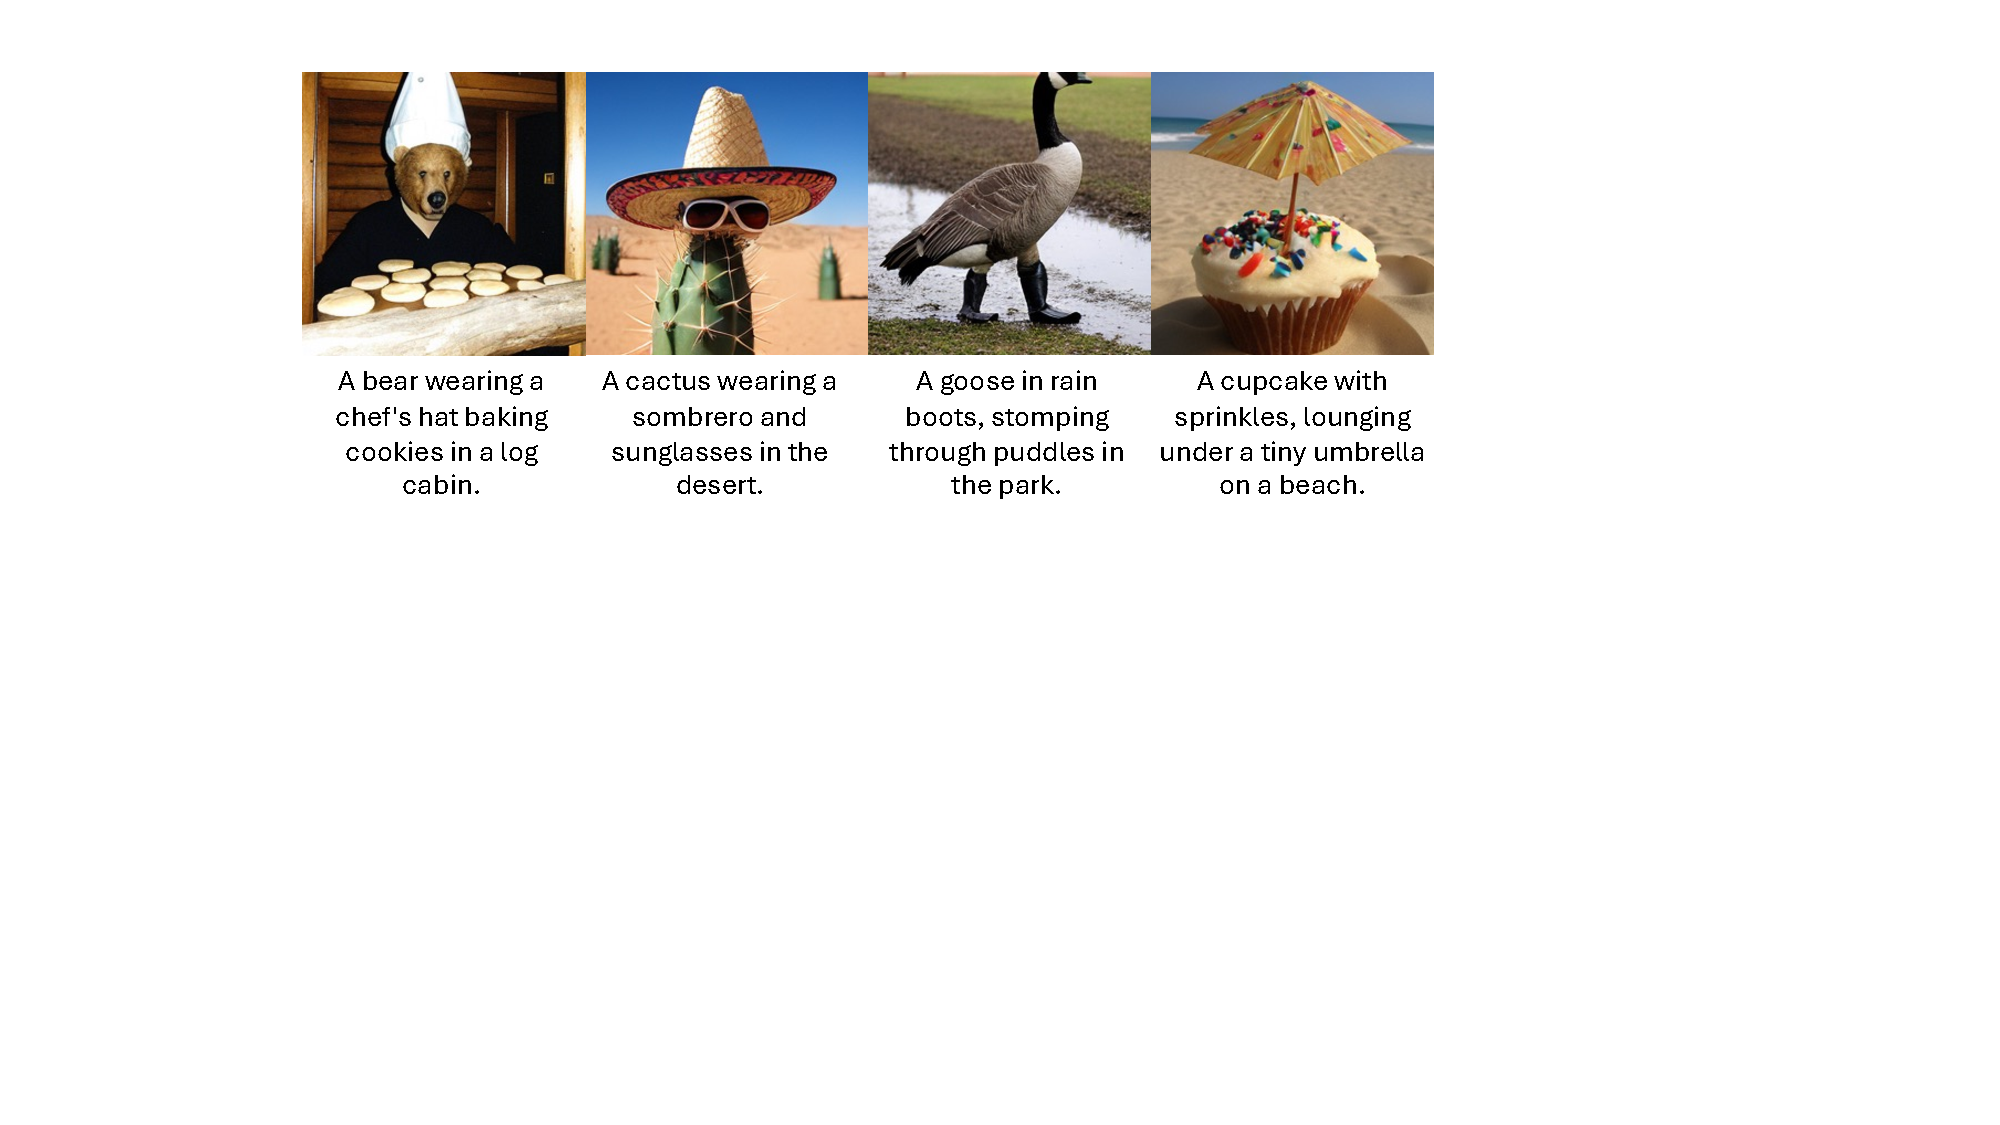
\includegraphics[width=\linewidth]{figs/t2i.pdf}
        \caption{Samples on Text-to-Image generation.}
        \label{fig:subfig1}
    \end{subfigure}

    \begin{subfigure}{1\textwidth}
        \centering
        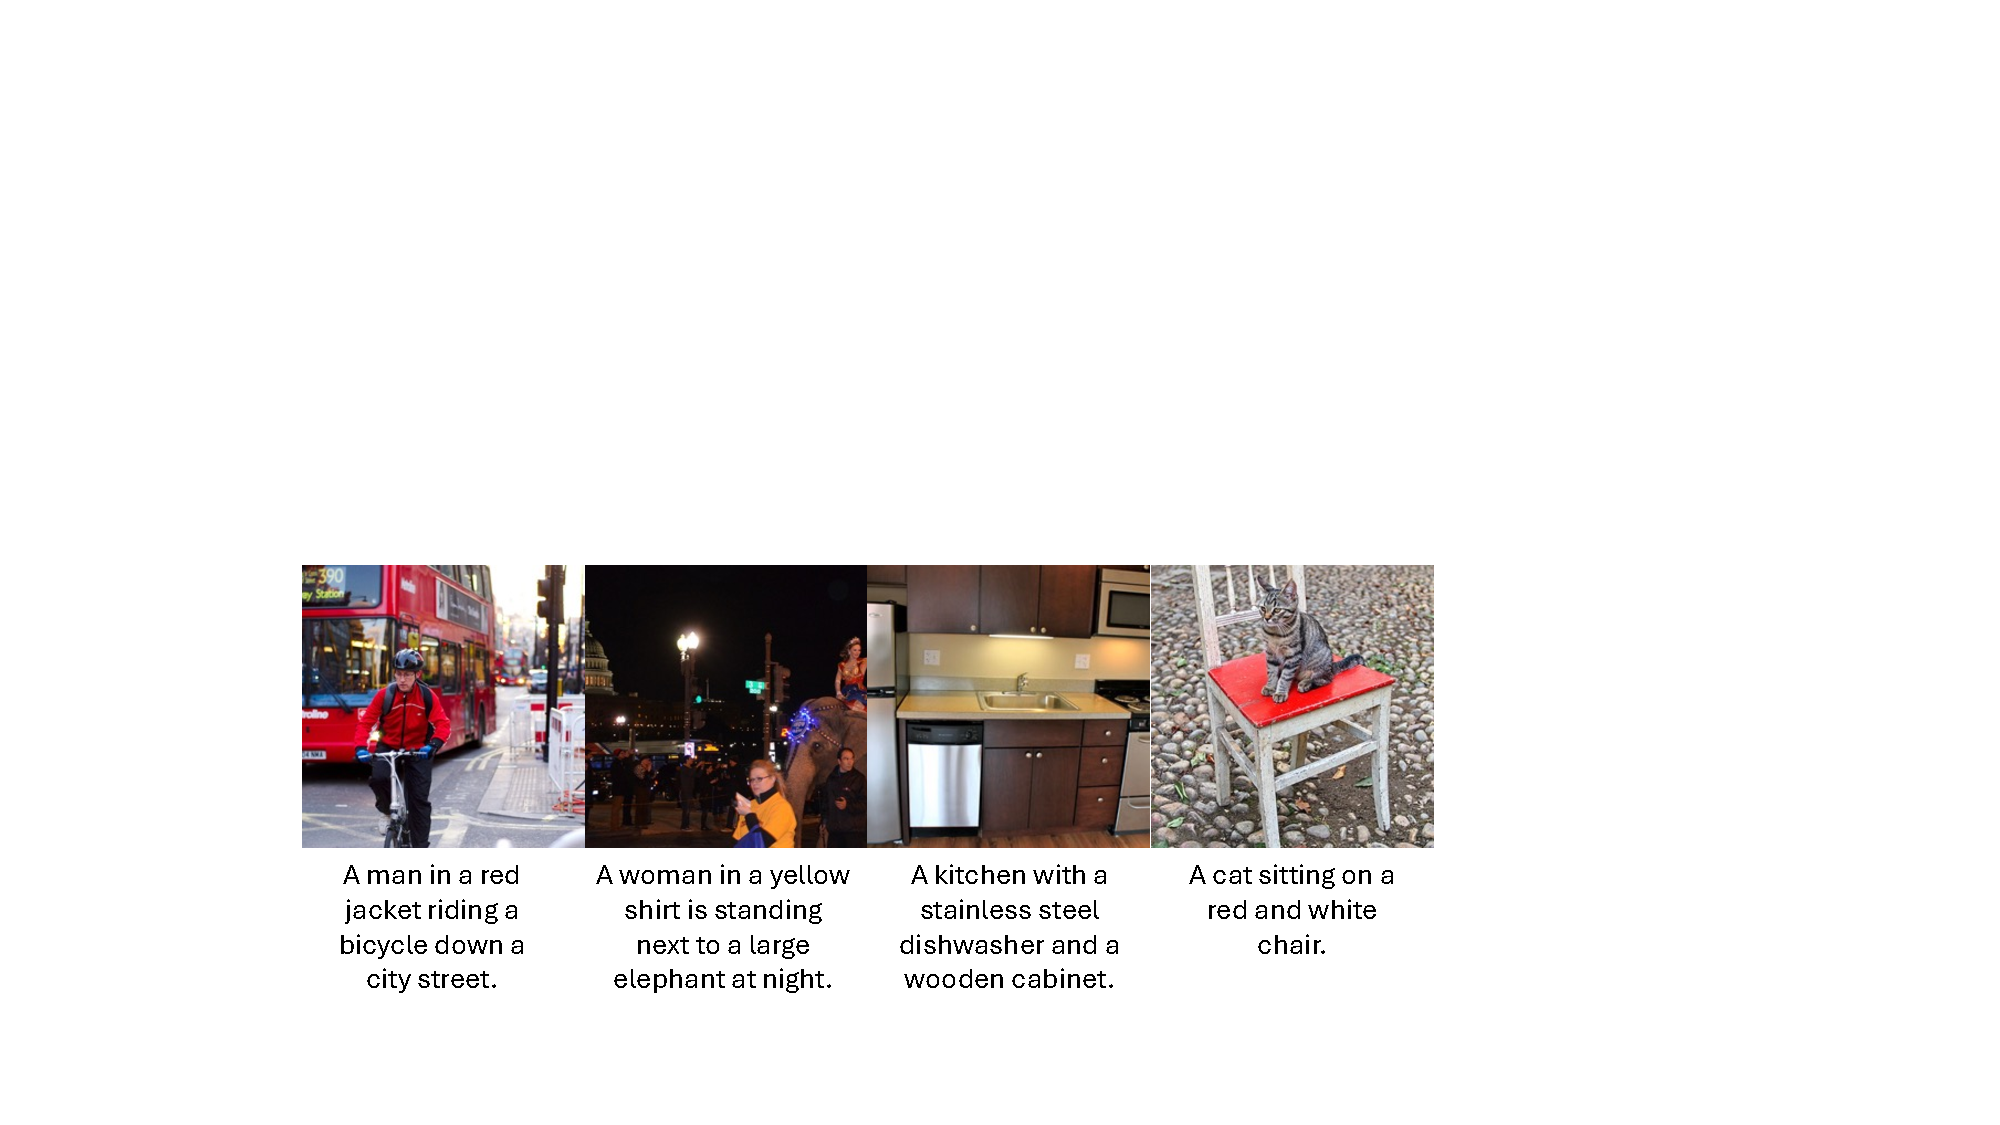
\includegraphics[width=\linewidth]{figs/i2t.pdf}
        \caption{Samples on Image Caption generation.     \vspace{-5pt}
        }
        \label{fig:subfig2}
    \end{subfigure}
    \vspace{-5pt}
    \caption{\textbf{Multimodal generation}. Results are generated by a single CausalFusion XL model trained on ImageNet recaption data.
    \vspace{-10pt}
    }
    \label{fig:combined}
\end{figure}



\begin{table*}[h!]
\footnotesize
\centering
\subfloat[MSCOCO~\cite{lin2014microsoft} is used for FID30k and CIDEr evalution.]{
\begin{tabular}{c|cc|cc}
  & Source & Size & FID30k$\downarrow$ & CIDEr$\uparrow$ \\
\shline
Transfusion-L~\cite{transfusion} & IN1KCap & 1M & 8.1 & 34.5 \\
CausalFusion-L & IN1KCap & 1M & \textbf{7.1} & \textbf{47.9} \\
\end{tabular}
}
\hfill
\subfloat[ImageNet is used for FID10k and Acc, MSCOCO is used for CIDEr evalution.]{
\begin{tabular}{c|c|cc|cc|c}
 & Params & Data & Size & FID10k$\downarrow$ & Acc$\uparrow$ &  CIDEr$\uparrow$ \\
\shline
DiT~\cite{dit} & 458M & IN1K & 1M & 18.2 & 83.5  & 94.4 \\
CausalFusion& 368M & IN1K & 1M & 11.8 & 84.2  & 98.0 \\
{CausalFusion}$^\dagger$ & 368M  & IN1K & 1M & \textbf{9.3} & \textbf{84.7} & \textbf{103.2} \\
\end{tabular}
}
\vspace{-5pt}
\caption{
(a) \textbf{Comparison with Transfusion}~\cite{transfusion} on perception and generation benchmarks. All models are trained under the same settings using the same pretraining data. (b) \textbf{Comparison with DiT}~\cite{dit} on perception and generation benchmarks. The model marked with $\dagger$ is trained with a VAE from \cite{mar}, using a loss function to predict latent variables rather than noise.
\vspace{-10pt}
}
\label{tab:multimodal}
\end{table*}

\vspace{-5pt}
\paragraph{Zero-shot image editing.}
CausalFusion naturally supports zero-shot image editing, as it is trained to predict a random subset of image tokens based on a random subset of visible image tokens. This inherent flexibility enables the model to perform localized edits without requiring task-specific fine-tuning. As shown in Figure~\ref{fig:vis1}(b), our model can generate high-quality editing results even when only pretrained on the ImageNet class-conditional generation task, demonstrating its robustness and adaptability to editing tasks. Moreover, CausalFusion's dual-factorized design allows it to balance contextual coherence with high-fidelity updates, ensuring that edited regions blend seamlessly into the surrounding content. See Appendix~\ref{appendix:secD} for additional visualizations showcasing the model's ability to handle diverse editing scenarios.


\vspace{-5pt}
\paragraph{Vision-Language joint modeling.}
CausalFusion can integrate the language modality by applying a separate next-token prediction loss on text, similar to GPT~\cite{gpt1}, enabling it to jointly model both image and text data. In this experiment, CausalFusion was trained on two tasks simultaneously: Text-to-Image (T2I) generation and Image Captioning. During training, text precedes the image in 90\% of cases, framing it as a T2I task where only the image loss is applied. In the remaining cases, the text follows the image, and both text loss (for Image Captioning) and image loss (for classifier-free guidance~\cite{ho2022classifier} in T2I) are applied, with the text loss weighted at 0.01 relative to the image loss.

We follow the configurations and training/inference protocols from previous sections. For language tokenization, we use the LLaMA-3~\cite{llama3} tokenizer. Models are trained on a re-captioned ImageNet dataset, with each image labeled by 10 captions generated by Qwen2VL-7B~\cite{qwen2vl}. T2I and Image Captioning tasks are evaluated using zero-shot MSCOCO-30k FID and zero-shot MSCOCO CIDEr on Karpathy's test split, respectively. We compare CausalFusion with a contemporary multimodal model, Transfusion~\cite{transfusion}, which integrates language and vision modeling using standard diffusion loss for images and next-token prediction loss for text. In Transfusion, language tokens are conditioned on image embeddings with added diffusion noise. As Transfusion is not open-sourced, we implemented it based on the original paper, aligning the model architecture, VAE encoder, and language tokenizer with those used in CausalFusion.
Results with 240-epoch training are presented in Table~\ref{tab:multimodal}(a). Compared to Transfusion, CausalFusion demonstrates superior performance in both text-to-image generation and image captioning, highlighting its strong potential as a foundational model for multimodal tasks. 
In Figure \ref{fig:combined}, we show a single pretrained CausalFusion XL model performing text-to-image generation at the top and image-to-text generation (image captioning) at the bottom. Further experiment details, including data, model design, and hyperparameters, are provided in Appendix~\ref{appendix:secC}.

\vspace{-5pt}
\paragraph{Visual Representation Learning.} We further evaluate CausalFusion models from a representation learning perspective. Specifically, we leverage the CausalFusion model pretrained on the 256$\times$256 ImageNet class-conditional generation task and fine-tune it on the ImageNet classification and MSCOCO captioning tasks. For image classification, we use the average-pooled features from the last layer of CausalFusion, followed by a linear classifier. For image captioning, we add a small transformer encoder-decoder module as the language head on top of CausalFusion.
The pretrained CausalFusion model follows the default configuration described in previous sections. We compare it to the DiT-L/2 model pretrained for the same number of epochs. Detailed hyperparameters for fine-tuning are provided in Appendix~\ref{appendix:secC}. 
As shown in Table~\ref{tab:multimodal}(b), our CausalFusion model outperforms DiT on all fine-tuning tasks, indicating that CausalFusion learns superior representations compared to DiT. We hypothesize that the random grouped token diffusion mechanism in CausalFusion, which diffuses images with partially observed inputs, implicitly performs as masked representation prediction \cite{he2022masked, maskedpredict}, enhancing the model's representation learning ability.
